\documentclass[11pt,a4paper]{article}

\usepackage[margin=2.5cm]{geometry}
\usepackage{booktabs}
\usepackage{float}
\usepackage{tabularx}
\usepackage{xltabular}
\usepackage{array}
\usepackage{enumitem}
\usepackage{totcount}
\usepackage{fancyhdr}
\usepackage{lastpage}
\usepackage{needspace}
\usepackage{tikz}
\usetikzlibrary{arrows.meta,positioning,fit,calc,shapes.geometric}
\usepackage[hidelinks]{hyperref}
\setlength{\emergencystretch}{1.5em}

% Section numbers in the same style as the ConOps: 1.0, 1.1.
\renewcommand{\thesection}{\arabic{section}.0}
\renewcommand{\thesubsection}{\arabic{section}.\arabic{subsection}}

% Controlled-document header on every page.
\newcommand{\docref}{Reference TBD}
\newcommand{\docrev}{Issue 1, Rev.~0 --- DRAFT}
\pagestyle{fancy}
\fancyhf{}
\lhead{\footnotesize Fail-Safe In-Orbit Reprogramming of a Spacecraft Controller --- Software Architecture}
\lfoot{\small \docref}
\cfoot{\small \docrev}
\rfoot{\small Page \thepage\ of \pageref{LastPage}}

% Open items. TBD = not known. TBR = proposal awaiting the author's
% acceptance. Listed in App. B; totals counted, not typed.
\newtotcounter{tbd}
\newtotcounter{tbr}
\newcommand{\tbditem}[2]{\refstepcounter{tbd}\label{tbd:#1}\item[TBD-\thetbd] #2}
\newcommand{\tbritem}[2]{\refstepcounter{tbr}\label{tbr:#1}\item[TBR-\thetbr] #2}
\newcommand{\tbd}[1]{\mbox{\textbf{[\hyperref[tbd:#1]{TBD-\ref*{tbd:#1}}]}}}
\newcommand{\tbr}[1]{\mbox{\textbf{[\hyperref[tbr:#1]{TBR-\ref*{tbr:#1}}]}}}

% A component box in Figure 1: name, then its role in small type.
\newcommand{\nohyph}{\hyphenpenalty=10000\exhyphenpenalty=10000\relax}
\newcommand{\cmp}[2]{#1\\[-1pt]{\scriptsize\color{black!70}#2}}

% Column head of an options table: hazard, with its severity beneath.
\newcommand{\sev}[2]{\begin{tabular}[b]{@{}c@{}}#1\\{\scriptsize #2}\end{tabular}}

% Run-in label for the parts of a design decision.
\newcommand{\field}[1]{\par\needspace{4\baselineskip}\smallskip\noindent\textbf{#1.}~}

\setlist[description]{style=multiline,leftmargin=2cm,nosep,font=\normalfont\bfseries}
\setlist[itemize]{nosep}

\begin{document}

\thispagestyle{fancy}
\begin{center}
{\LARGE\bfseries Fail-Safe In-Orbit Reprogramming\\[0.2em] of a Spacecraft Controller\par}
\vspace{0.4em}
{\Large Software Architecture\par}
\vspace{1em}
\begin{tabular}{@{}ll@{}}
Reference & TBD \tbd{ref} \\
Issue / revision & Issue 1, Revision 0 --- DRAFT \\
Date & 11 October 2026 \\
Author & Andrew Toma \\
Open items & \total{tbd} TBD, \total{tbr} TBR (App.~A) \\
\end{tabular}
\end{center}

\subsection*{Document change record}
\begin{tabular}{@{}llll@{}}
\toprule
Issue & Rev. & Date & Change \\
\midrule
1 & 0 & 2026-10-11 & First draft \\
\bottomrule
\end{tabular}

% ===========================================================================
\section{Purpose and Scope}
This document records the software architecture of the System: its
components, what each does, how they connect, and the design decisions behind
them [1,~Sec.~4.2.3, p.~33]. It covers the three software items of the
requirements [6,~Sec.~3.1].

The architecture concentrates on ``the most pressing risks'' [3,~Sec.~4]: the
eight catastrophic and critical hazards that do not yet meet the fault
tolerance rule [5,~Sec.~5.0]. The software qualities it is built for are the
two a high-risk project emphasises, fault tolerance and security
[3,~Sec.~4], and the testability the requirements demand.

The architecture remains strictly hardware-agnostic, defining functional
component behavior rather than the hardware that executes it, and concludes
with the capabilities the hardware must provide. Detailed component designs,
including specific algorithms and data structures, are documented before each
component is implemented [1,~Sec.~4.3.2, p.~34].

\noindent\textbf{How to read it.} Section~\ref{sec:overview} shows every
component and one update on two figures. Section~\ref{sec:decisions} holds the design
decisions, each with the options weighed and the hazards it targets.
Section~\ref{sec:components} gives each component's role and the requirements
it meets. Section~\ref{sec:hardware} lists what the hardware must provide.

% ===========================================================================
\section{Documents}
\noindent [1] NASA, \emph{NASA Software Engineering Requirements}, NPR 7150.2D.

\noindent [2] NASA, \emph{NASA Software Engineering Handbook}, NASA-HDBK-2203,
Version~D, Topic 5.13 ``SwDD -- Software Design Description''.

\noindent [3] NASA, \emph{NASA Software Engineering Handbook}, NASA-HDBK-2203,
Version~D, SWE-057 ``Software Architecture''.

\noindent [4] \emph{Fail-Safe In-Orbit Reprogramming of a Spacecraft
Controller --- Concept of Operations}, Issue~1, Revision~1, Draft.

\noindent [5] \emph{Fail-Safe In-Orbit Reprogramming of a Spacecraft
Controller --- Hazard Analysis}, Issue~1, Revision~0, Draft.

\noindent [6] \emph{Fail-Safe In-Orbit Reprogramming of a Spacecraft
Controller --- Software Requirements Specification}, Issue~1, Revision~0,
Draft.

\noindent [7] \emph{Fail-Safe In-Orbit Reprogramming of a Spacecraft
Controller --- Software Classification}, Issue~1, Revision~1, Draft.

\noindent [8] NASA, \emph{NASA Software Safety Guidebook}, NASA-GB-8719.13,
2004.

\noindent [9] MCUboot project, \emph{Bootloader} design document,
\texttt{docs/design.md}, commit 1d2643c, 11 September 2026.

\noindent [10] G.~Reeves and T.~Neilson, ``The Mars Rover Spirit FLASH
Anomaly'', IEEE Aerospace Conference, paper 1426, 2005.

\noindent [11] NASA, \emph{Space System Protection Standard}, NASA-STD-1006A,
15 July 2022.

\noindent [12] NASA, \emph{Fault Management Handbook}, NASA-HDBK-1002,
Draft~2, 2 April 2012. A draft, not a released standard.

\noindent [13] MCUboot project, \emph{Serial recovery},
\texttt{docs/serial\_recovery.md}, commit 1d2643c, 11 September 2026.

% ===========================================================================
\section{System Overview}
\label{sec:overview}
The System has three software items [6,~Sec.~3.1], each made of components
(Figure~\ref{fig:overview}). The ground software builds and checks
the operator's commands, singly or as a planned sequence. It checks each
firmware release the operator approves, encrypts and signs it, and checks the
signed result before sending it. It keeps every report that comes back. The onboard computer software checks everything that arrives and passes
it on; between contacts it stores the controller's reports, watches the
controller, and restores it when no firmware can run. The controller firmware
acts on commands, reports its state and handles its own faults. It tries new
firmware before keeping it and returns to working firmware on its own when the
new firmware fails: a bootloader chooses which copy runs, and the
last-resort firmware takes over when the main firmware cannot.
Figure~\ref{fig:update} follows one update from release to confirmed firmware.

\begin{figure}[H]
\centering
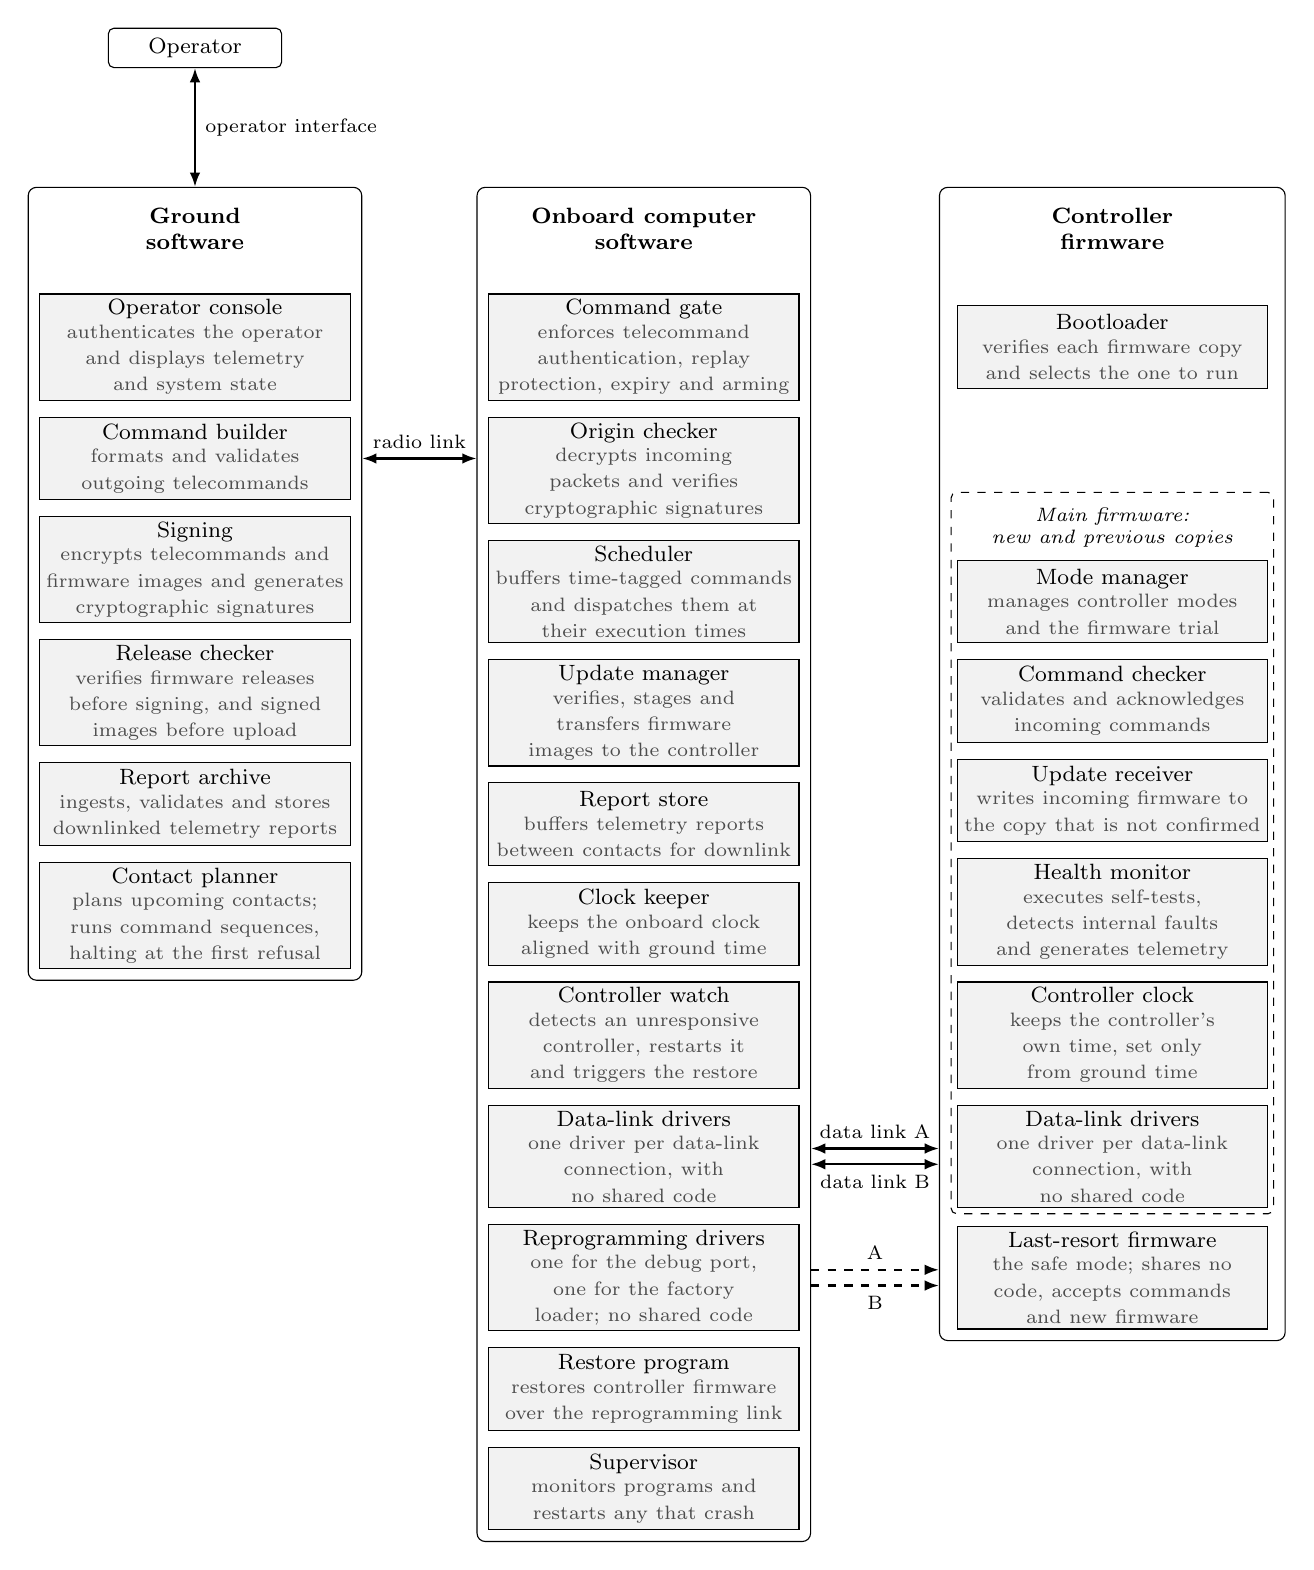
\begin{tikzpicture}[
  font=\footnotesize,
  comp/.style={draw, fill=black!5, text width=3.8cm, minimum height=1.05cm, inner sep=2pt, align=center,
    execute at begin node=\nohyph},
  title/.style={font=\footnotesize\bfseries, align=center},
  item/.style={draw, rounded corners=3pt, inner sep=4pt},
  link/.style={{Latex[length=1.8mm]}-{Latex[length=1.8mm]}, thick},
  lab/.style={font=\scriptsize, align=center},
]
% Ground software: boxes stacked with an even gap
\node[title] (gt) at (0,1.5) {Ground\\software};
\node[comp] (g1) at (0,0) {\cmp{Operator console}{authenticates the operator and displays telemetry and system state}};
\node[comp, below=0.2cm of g1] (g2) {\cmp{Command builder}{formats and validates outgoing telecommands}};
\node[comp, below=0.2cm of g2] (g3) {\cmp{Signing}{encrypts telecommands and firmware images and generates cryptographic signatures}};
\node[comp, below=0.2cm of g3] (g4) {\cmp{Release checker}{verifies firmware releases before signing, and signed images before upload}};
\node[comp, below=0.2cm of g4] (g5) {\cmp{Report archive}{ingests, validates and stores downlinked telemetry reports}};
\node[comp, below=0.2cm of g5] (g6) {\cmp{Contact planner}{plans upcoming contacts; runs command sequences, halting at the first refusal}};
\node[item, fit=(gt)(g1)(g6)] (gbox) {};

% Onboard computer software
\node[title] (ot) at (5.7,1.5) {Onboard computer\\software};
\node[comp] (o1) at (5.7,0) {\cmp{Command gate}{enforces telecommand authentication, replay protection, expiry and arming}};
\node[comp, below=0.2cm of o1] (o2) {\cmp{Origin checker}{decrypts incoming packets and verifies cryptographic signatures}};
\node[comp, below=0.2cm of o2] (o3) {\cmp{Scheduler}{buffers time-tagged commands and dispatches them at their execution times}};
\node[comp, below=0.2cm of o3] (o4) {\cmp{Update manager}{verifies, stages and transfers firmware images to the controller}};
\node[comp, below=0.2cm of o4] (o5) {\cmp{Report store}{buffers telemetry reports between contacts for downlink}};
\node[comp, below=0.2cm of o5] (o6) {\cmp{Clock keeper}{keeps the onboard clock aligned with ground time}};
\node[comp, below=0.2cm of o6] (o7) {\cmp{Controller watch}{detects an unresponsive controller, restarts it and triggers the restore}};
\node[comp, below=0.2cm of o7] (o8) {\cmp{Data-link drivers}{one driver per data-link connection, with no shared code}};
\node[comp, below=0.2cm of o8] (o9) {\cmp{Reprogramming drivers}{one for the debug port, one for the factory loader; no shared code}};
\node[comp, below=0.2cm of o9] (o10) {\cmp{Restore program}{restores controller firmware over the reprogramming link}};
\node[comp, below=0.2cm of o10] (o11) {\cmp{Supervisor}{monitors programs and restarts any that crash}};
\node[item, fit=(ot)(o1)(o11)] (obox) {};

% Controller firmware: the data-link drivers face those of the onboard computer
\node[title] (ct) at (11.65,1.5) {Controller\\firmware};
\node[comp] (c0) at (11.65,0) {\cmp{Bootloader}{verifies each firmware copy and selects the one to run}};
\node[comp] at (o8 -| c0) (m6) {\cmp{Data-link drivers}{one driver per data-link connection, with no shared code}};
\node[comp, above=0.2cm of m6] (m5) {\cmp{Controller clock}{keeps the controller's own time, set only from ground time}};
\node[comp, above=0.2cm of m5] (m4) {\cmp{Health monitor}{executes self-tests, detects internal faults and generates telemetry}};
\node[comp, above=0.2cm of m4] (m3) {\cmp{Update receiver}{writes incoming firmware to the copy that is not confirmed}};
\node[comp, above=0.2cm of m3] (m2) {\cmp{Command checker}{validates and acknowledges incoming commands}};
\node[comp, above=0.2cm of m2] (m1) {\cmp{Mode manager}{manages controller modes and the firmware trial}};
\node[font=\scriptsize\itshape, align=center, above=1pt of m1] (mt) {Main firmware:\\new and previous copies};
\node[draw, dashed, rounded corners=2pt, inner sep=2pt, fit=(mt)(m1)(m6)] (main) {};
\node[comp] at (o9 -| c0) (c9) {\cmp{Last-resort firmware}{the safe mode; shares no code, accepts commands and new firmware}};
\node[item, fit=(ct)(c0)(main)(c9)] (cbox) {};

% Operator
\node[draw, rounded corners=2pt, minimum width=2.2cm, minimum height=0.5cm] (op) at (0,3.8) {Operator};
\draw[link] (op.south) -- (gbox.north) node[midway, right, lab] {operator interface};

% Links
\draw[link] (g2.east -| gbox.east) -- (g2.east -| obox.west) node[midway, above, lab] {radio link};
\draw[link] ($(o8.east -| obox.east)+(0,0.1)$) -- ($(m6.west -| cbox.west)+(0,0.1)$)
  node[midway, above, lab] {data link A};
\draw[link] ($(o8.east -| obox.east)+(0,-0.1)$) -- ($(m6.west -| cbox.west)+(0,-0.1)$)
  node[midway, below, lab] {data link B};
\draw[-{Latex[length=1.8mm]}, thick, dashed] ($(o9.east -| obox.east)+(0,0.1)$) -- ($(o9.east -| cbox.west)+(0,0.1)$)
  node[midway, above, lab] {A};
\draw[-{Latex[length=1.8mm]}, thick, dashed] ($(o9.east -| obox.east)+(0,-0.1)$) -- ($(o9.east -| cbox.west)+(0,-0.1)$)
  node[midway, below, lab] {B};
\end{tikzpicture}
\caption{The three software items and their components. The data link and the
reprogramming link each have two independent connections, A and B. The dashed
arrows are the reprogramming link, which reaches the controller whatever its
memory holds.}
\label{fig:overview}
\end{figure}

\begin{figure}[H]
\centering
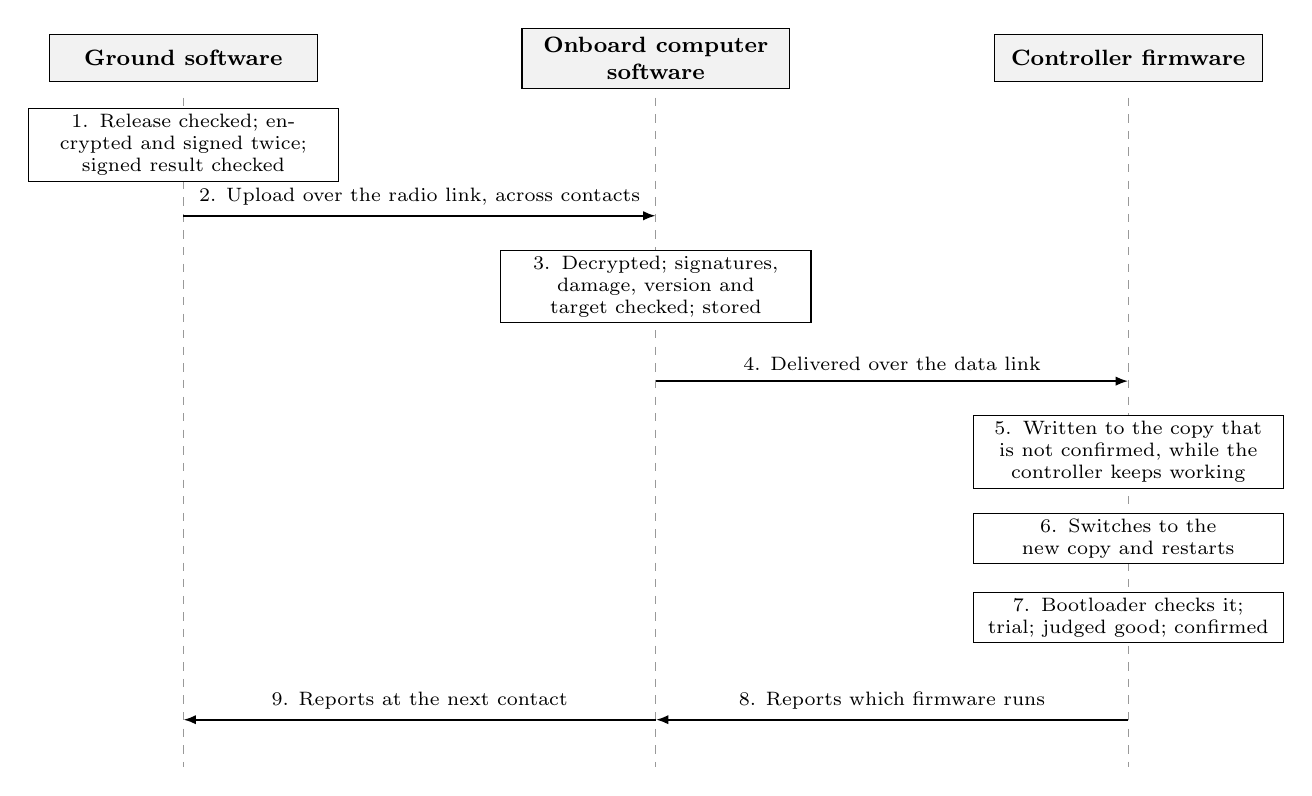
\begin{tikzpicture}[font=\scriptsize,
  head/.style={draw, fill=black!5, minimum width=3.4cm, minimum height=0.6cm, font=\footnotesize\bfseries, align=center},
  act/.style={draw, fill=white, text width=3.8cm, align=center, inner sep=2pt},
  msg/.style={-{Latex[length=1.6mm]}, thick}]
\node[head] at (0,0) {Ground software};
\node[head] at (6,0) {Onboard computer\\software};
\node[head] at (12,0) {Controller firmware};
\foreach \x in {0,6,12} \draw[dashed, black!40] (\x,-0.5) -- (\x,-9.0);
\node[act] at (0,-1.1) {1. Release checked; encrypted and signed twice; signed result checked};
\draw[msg] (0,-2.0) -- node[above]{2. Upload over the radio link, across contacts} (6,-2.0);
\node[act] at (6,-2.9) {3. Decrypted; signatures, damage, version and target checked; stored};
\draw[msg] (6,-4.1) -- node[above]{4. Delivered over the data link} (12,-4.1);
\node[act] at (12,-5.0) {5. Written to the copy that is not confirmed, while the controller keeps working};
\node[act] at (12,-6.1) {6. Switches to the new copy and restarts};
\node[act] at (12,-7.1) {7. Bootloader checks it; trial; judged good; confirmed};
\draw[msg] (12,-8.4) -- node[above]{8. Reports which firmware runs} (6,-8.4);
\draw[msg] (6,-8.4) -- node[above]{9. Reports at the next contact} (0,-8.4);
\end{tikzpicture}
\caption{One update, from release to confirmed firmware. If the trial fails,
the controller returns to the previous copy (Figure~\ref{fig:startup}).}
\label{fig:update}
\end{figure}

% ===========================================================================
\section{Constraints}
Three constraints of the ConOps change the design [4,~Secs.~1.1.2 and 8.0].
\begin{description}
\item[C-3] System development is conducted by a single engineer. Component
  independence is achieved through isolated software codebases rather than
  organizational team separation; one engineer writing every codebase limits
  their diversity.
\item[R-4] The space segment relies on a single onboard computer. A spacecraft
  can carry a second, redundant one, as the Mars Reconnaissance Orbiter does
  [12,~App.~F.2.15, Lesson 2041, p.~197]; how many is a spacecraft decision,
  outside this project. Its permanent failure halts command handling,
  telemetry reporting and firmware restoration. This single-point failure risk
  is formally accepted, so H-4 does not meet the fault tolerance rule
  [5,~Sec.~5.2].
\item[C-4] The onboard computer software and the controller firmware execute on
  two given development boards. The architectural design remains
  hardware-agnostic, with board compatibility evaluated separately at the end of
  this document.
\end{description}

% ===========================================================================
\section{Design Decisions}
\label{sec:decisions}
Each decision targets hazards that do not yet meet the fault tolerance rule
[5,~Sec.~5.2]. It states the problem, weighs the options, and lists the
requirements the choice adds; these enter the requirements at their next
revision. Where a proven design exists, it is one of the options
[3,~Sec.~4].

Options are compared by the smallest number of failures that, together, cause
the hazard with that option in place. A catastrophic hazard needs at least three, a
critical one two [5,~Sec.~3.3]. The counts leave out the permanent loss
of the onboard computer, an accepted risk (R-4). They are design targets, which
the hazard analysis confirms in its design phase [5,~Sec.~1.0]. In each
options table, the last column marks the option the decision picks (YES) and
the options it rejects (NO).

% ---------------------------------------------------------------- 5.1
\needspace{9\baselineskip}
\subsection{Start-Up and Fall-Back}
\label{sec:startup}
\field{Problem} Every firmware copy is started by the same bootloader and
depends on the data it keeps over restarts. A defect in the bootloader, or kept
data it cannot handle, stops every copy, and today's restore writes back the
same bootloader, so the defect returns [5,~Sec.~5.2]. One failure is then
enough for H-8, the controller stopping between contacts with nothing on board
to bring it back, and for H-1, the controller left with no firmware it can run
and no way to restore it.

\smallskip
{\small\noindent\begin{tabularx}{\textwidth}{@{}l>{\raggedright\arraybackslash}Xcc@{}}
\toprule
 & Option & \sev{H-8}{CRITICAL} & Chosen \\
\midrule
a & No bootloader: the last-resort firmware is the first code to run and decides which copy runs. A defect in it stops every start, and the restore puts the same firmware back, so the controller stays down until the ground loads a correction at the next contact. & 1 & NO \\
b & MCUboot's design [9,~Sec.~Boot Swap Types]: a small bootloader runs first, runs a new copy as a test and returns to the old copy unless the new one confirms itself. It survives a defect in any copy, but not one in the bootloader itself: that stops every start, and the restore writes the same bootloader back. & 1 & NO \\
c & Option b, plus a last-resort firmware sharing no code with the bootloader or the copies. When the bootloader fails, the controller goes silent and the onboard computer restores it, putting the last-resort firmware where the bootloader was, so it runs first (Figure~\ref{fig:memory}). The controller stays down only if a second failure follows: a defect in the last-resort firmware, or a failed restore. & 2 & YES \\
\bottomrule
\end{tabularx}}


\field{Choice} Option c, shown in Figures~\ref{fig:startup} and
\ref{fig:memory}. It keeps MCUboot's test and revert, which exists to keep bad
firmware from leaving a device unusable [9,~Sec.~Boot Swap Types], and adds a
last-resort firmware sharing no code with the rest [6,~REQ-009]. The
last-resort firmware is the controller's safe mode: it still accepts commands
from the ground [12,~Sec.~6.4.3.2.4, p.~85]. H-1, which also needs the
ground's way in, is decided in Section~\ref{sec:wayback}.

\begin{figure}[H]
\centering
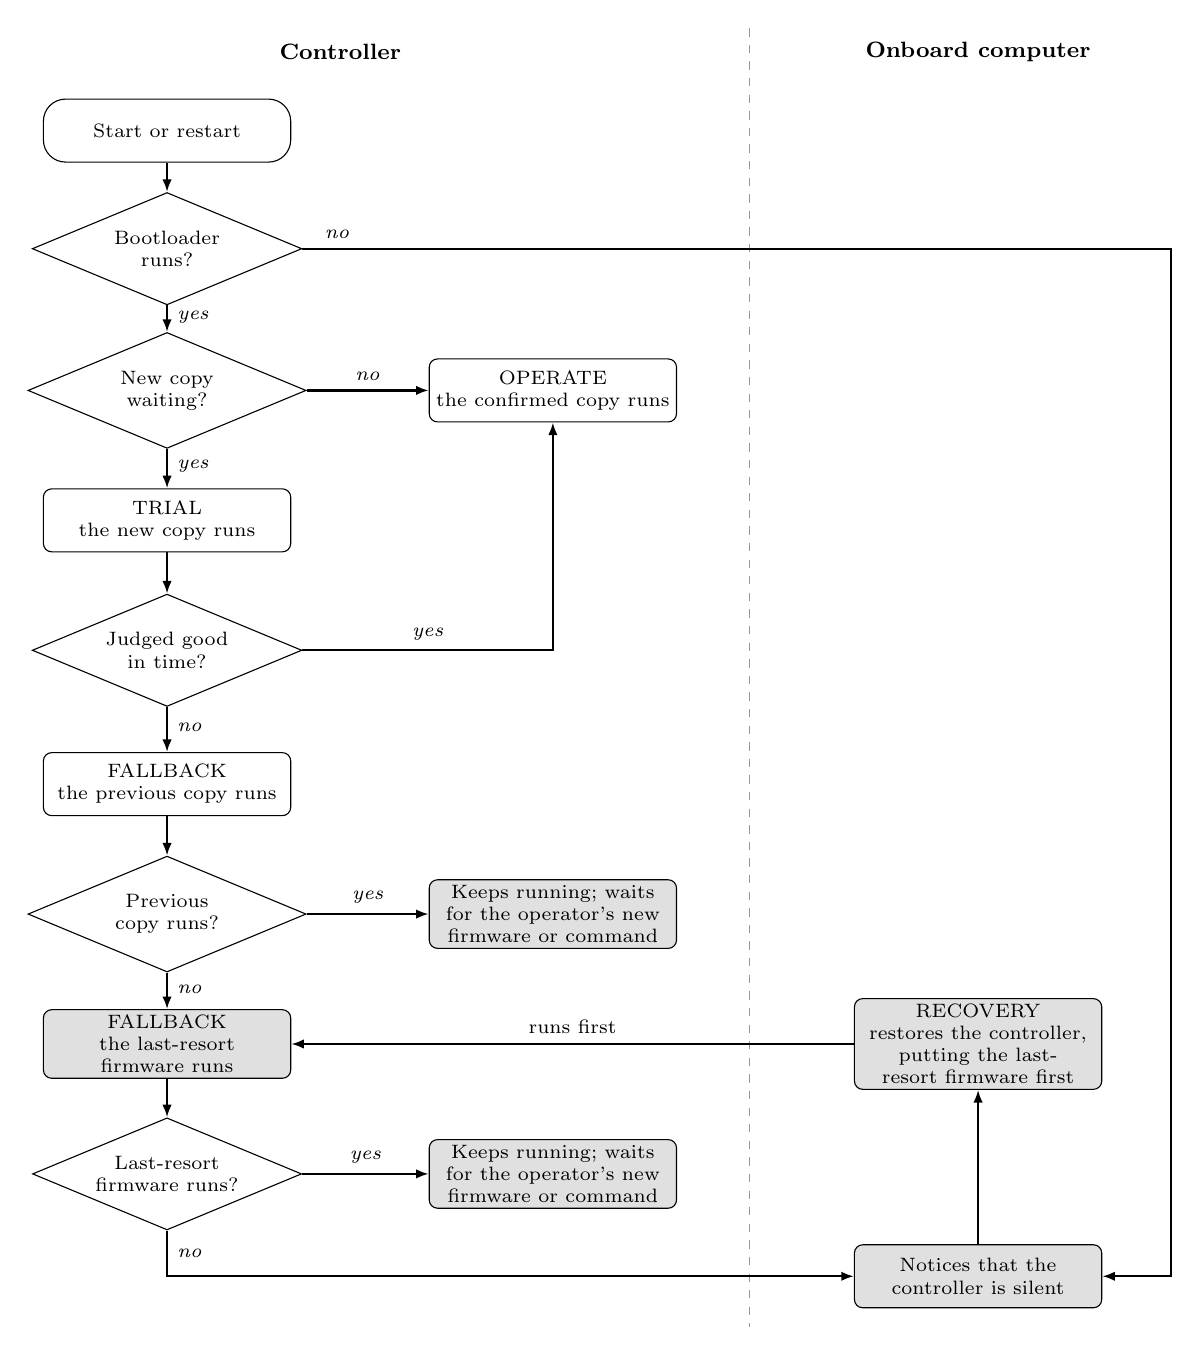
\begin{tikzpicture}[font=\scriptsize,
  box/.style={draw, rounded corners=3pt, text width=3.0cm, align=center, minimum height=0.8cm, inner sep=2pt},
  add/.style={box, fill=black!12},
  ask/.style={draw, diamond, aspect=2.4, inner sep=1pt, align=center, text width=2.1cm},
  tr/.style={-{Latex[length=1.6mm]}, thick},
  yn/.style={font=\scriptsize\itshape}]
% Lanes
\node[font=\footnotesize\bfseries] at (2.2,1.0) {Controller};
\node[font=\footnotesize\bfseries] at (10.3,1.0) {Onboard computer};
\draw[dashed, black!40] (7.4,1.3) -- (7.4,-15.2);
% Controller lane
\node[box, rounded corners=8pt] (start) at (0,0) {Start or restart};
\node[ask] (d1) at (0,-1.5) {Bootloader runs?};
\node[ask] (d2) at (0,-3.3) {New copy waiting?};
\node[box] (trial) at (0,-4.95) {TRIAL\\the new copy runs};
\node[ask] (d3) at (0,-6.6) {Judged good in time?};
\node[box] (prev) at (0,-8.3) {FALLBACK\\the previous copy runs};
\node[ask] (d4) at (0,-9.95) {Previous copy runs?};
\node[add] (lr) at (0,-11.6) {FALLBACK\\the last-resort firmware runs};
\node[ask] (d5) at (0,-13.25) {Last-resort firmware runs?};
\node[box] (op) at (4.9,-3.3) {OPERATE\\the confirmed copy runs};
\node[add] (w1) at (4.9,-9.95) {Keeps running; waits for the operator's new firmware or command};
\node[add] (w2) at (4.9,-13.25) {Keeps running; waits for the operator's new firmware or command};
% Onboard computer lane
\node[add] (seen) at (10.3,-14.55) {Notices that the controller is silent};
\node[add] (rec) at (10.3,-11.6) {RECOVERY\\restores the controller, putting the last-resort firmware first};
% Flow
\draw[tr] (start) -- (d1);
\draw[tr] (d1) -- node[pos=0.45, right, yn]{yes} (d2);
\draw[tr] (d2) -- node[above, yn]{no} (op);
\draw[tr] (d2) -- node[pos=0.45, right, yn]{yes} (trial);
\draw[tr] (trial) -- (d3);
\draw[tr] (d3.east) -| node[pos=0.25, above, yn]{yes} (op.south);
\draw[tr] (d3) -- node[pos=0.45, right, yn]{no} (prev);
\draw[tr] (prev) -- (d4);
\draw[tr] (d4) -- node[above, yn]{yes} (w1);
\draw[tr] (d4) -- node[pos=0.45, right, yn]{no} (lr);
\draw[tr] (lr) -- (d5);
\draw[tr] (d5) -- node[above, yn]{yes} (w2);
\draw[tr] (d5.south) |- node[pos=0.25, right, yn]{no} (seen.west);
\draw[tr] (d1.east) -- (12.75,-1.5) node[pos=0.04, above, yn]{no} |- (seen.east);
\draw[tr] (seen) -- (rec);
\draw[tr] (rec) -- node[above]{runs first} (lr);
\end{tikzpicture}
\caption{Start-up and fall-back as a flow. Each diamond is a check with a yes
and a no exit; a hang or too many failed starts counts as no. White: the
two-copy test and revert of MCUboot [9,~Sec.~Boot Swap Types]. Grey: added for
a controller that nobody can reach: the last-resort firmware, the wait for the
operator after a fall-back [6,~REQ-117], and the restore by the onboard
computer.}
\label{fig:startup}
\end{figure}

{\itshape\noindent\textbf{Note.} The restore is how the onboard computer brings back a
controller that runs no firmware. Through the reprogramming link, and without
using any controller software, it restarts the controller, writes its own copy
of the last-resort firmware into the place the controller starts from, clears
the kept data and starts the controller again. It tells the ground at the next
contact [6,~REQ-054 to REQ-060].\par}

\begin{figure}[H]
\centering
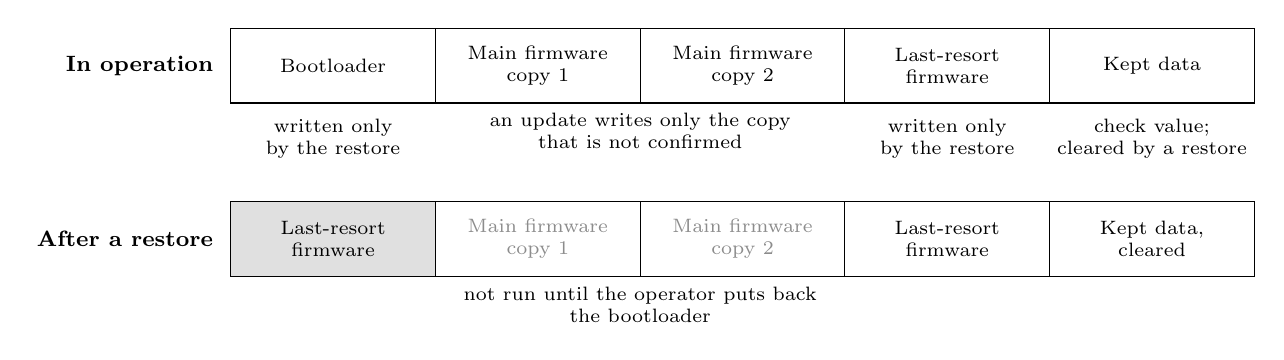
\begin{tikzpicture}[font=\scriptsize,
  cell/.style={draw, minimum width=2.6cm, minimum height=0.95cm, text width=2.4cm, align=center, inner sep=1pt},
  addc/.style={cell, fill=black!12},
  idle/.style={cell, text=black!45},
  row/.style={anchor=east, font=\footnotesize\bfseries, align=right}]
\node[row] at (-0.1,0) {In operation};
\node[cell] (a0) at (1.3,0) {Bootloader};
\node[cell] (a1) at (3.9,0) {Main firmware\\copy 1};
\node[cell] (a2) at (6.5,0) {Main firmware\\copy 2};
\node[cell] (a3) at (9.1,0) {Last-resort\\firmware};
\node[cell] (a4) at (11.7,0) {Kept data};
\node[below=2pt of a0, align=center] {written only\\by the restore};
\node[align=center] at ($(a1.south)!0.5!(a2.south)+(0,-0.35)$) {an update writes only the copy\\that is not confirmed};
\node[below=2pt of a3, align=center] {written only\\by the restore};
\node[below=2pt of a4, align=center] {check value;\\cleared by a restore};
\node[row] at (-0.1,-2.2) {After a restore};
\node[addc] (b0) at (1.3,-2.2) {Last-resort\\firmware};
\node[idle] (b1) at (3.9,-2.2) {Main firmware\\copy 1};
\node[idle] (b2) at (6.5,-2.2) {Main firmware\\copy 2};
\node[cell] (b3) at (9.1,-2.2) {Last-resort\\firmware};
\node[cell] (b4) at (11.7,-2.2) {Kept data,\\cleared};
\node[align=center] at ($(b1.south)!0.5!(b2.south)+(0,-0.35)$) {not run until the operator puts back\\the bootloader};
\end{tikzpicture}
\caption{The controller's memory, not to scale. After a restore, the
last-resort firmware (grey) sits in the bootloader's place and runs
first.}
\label{fig:memory}
\end{figure}

\field{Adds}
\begin{itemize}
\item The bootloader shall share no code with the main firmware or the
  last-resort firmware.
\item The restore shall put the last-resort firmware in the bootloader's
  place, so that it runs first.
\item The onboard computer software shall put back the bootloader and
  the main firmware through the reprogramming link when the operator orders it.
\end{itemize}

% ---------------------------------------------------------------- 5.2
\needspace{9\baselineskip}
\subsection{The Way Back In}
\label{sec:wayback}
\field{Problem} When the bootloader is broken (Section~\ref{sec:startup}),
the controller runs nothing, and only a restore can bring it back. A restore
that needed any software on the controller to receive it would fail at exactly
that moment, which the requirements forbid [6,~REQ-056]. The restore therefore
needs a way into the controller's memory that works with nothing running on
it, and the ground needs the same way in to load corrected firmware
[6,~REQ-058]. Targets H-1, the controller left with no firmware it can run and
no way to restore it. The same way in also serves H-3 and H-4.

\smallskip
{\small\noindent\begin{tabularx}{\textwidth}{@{}l>{\raggedright\arraybackslash}Xcc@{}}
\toprule
 & Option & \sev{H-1}{CATASTROPHIC} & Chosen \\
\midrule
a & The controller is asked to restore itself, as in MCUboot's serial recovery, which runs inside the bootloader [13,~Sec.~Entering Serial Recovery Mode]. A broken bootloader means nothing receives the order and nothing can load a correction. & 1 & NO \\
b & One separate way in that needs nothing running on the controller; the onboard computer drives it and can restart the controller. A broken bootloader is bypassed, but if this way in also breaks, nothing reaches the controller. & 2 & NO \\
c & Two separate ways in that share nothing: the controller's debug port, which writes memory directly with the processor stopped, and its factory loader, which a boot pin starts instead of our bootloader. A broken bootloader and one broken way in still leave the other. Each way in has its own driver on the onboard computer; a defect in the restore program that uses both is corrected by the system outside this project (A-6), as for H-3. & 3 & YES \\
\bottomrule
\end{tabularx}}


\field{Choice} Option c \tbr{wayback}. It follows the principle of hardware
commands, which a spacecraft executes on receipt without any flight software
[11,~Sec.~3.2, p.~9]. Such a command let the Spirit rover's team regain control
while its flight software kept resetting: it made the software start without
its flash memory [10,~pp.~4 and 9]. Two ways in are the fewest that meet the
rule. They still share the controller's memory and its reset wire; the hazard
analysis counts these shared causes when it is re-run on this design.

\field{Adds}
\begin{itemize}
\item The reprogramming link shall have two connections, independent of each
  other: the controller's debug port and its factory loader, each able to load
  the controller's memory whatever that memory holds.
\item The onboard computer software shall drive the debug port and the factory
  loader with separate drivers that share no code.
\item The onboard computer software shall be able to restart the controller.
\item No controller firmware shall be able to disable the debug port or the
  factory loader.
\end{itemize}

% ---------------------------------------------------------------- 5.3
\needspace{9\baselineskip}
\subsection{Restore Apart From Update}
\label{sec:apart}
\field{Problem} New firmware can reach the controller in two ways. In the
normal update, the onboard computer sends it over the data link to the
controller's running firmware, which writes it into memory. In the restore,
the onboard computer writes it into the controller's memory itself, through the
reprogramming link [6,~REQ-058]. Both start on the onboard computer, from a
copy of the firmware stored there. If one program did both jobs from one stored
copy, a single defect in that program, or a single damaged copy, would block
both ways at once. New firmware could then reach the controller only after the
system outside this project corrects the onboard computer's software (A-6)
[5,~Sec.~5.2]. Targets H-3, new firmware no longer able to reach the
controller.

\smallskip
{\small\noindent\begin{tabularx}{\textwidth}{@{}l>{\raggedright\arraybackslash}Xcc@{}}
\toprule
 & Option & \sev{H-3}{CATASTROPHIC} & Chosen \\
\midrule
a & One program does both the update and the restore, and both read the same stored copy of the firmware. One defect in that program, or damage to that copy, blocks both ways; the only barrier left is the outside system correcting the onboard computer (A-6). & 2 & NO \\
b & Two separate programs, the update manager and the restore program, each with its own code and its own stored copy of the firmware. Blocking both ways takes a defect in each program, and the outside correction failing as well. & 3 & YES \\
\bottomrule
\end{tabularx}}


\field{Choice} Option b \tbr{apart}. The two programs share nothing that one defect
could reach: when the update fails, the restore still works, and the other way
round.

\field{Adds}
\begin{itemize}
\item The restore program shall share no code or stored data with the update
  manager.
\end{itemize}

% ---------------------------------------------------------------- 5.4
\needspace{9\baselineskip}
\subsection{Proof of Origin}
\label{sec:origin}
\field{Problem} One means proves that both commands and firmware come from the
operator. If it is disclosed, another party can command the controller and
load firmware [5,~Sec.~5.2]. Targets H-2, firmware from someone else running
on the controller, and H-5, someone else commanding the System.

\smallskip
{\small\noindent\begin{tabularx}{\textwidth}{@{}l>{\raggedright\arraybackslash}Xccc@{}}
\toprule
 & Option & \sev{H-2}{CATASTROPHIC} & \sev{H-5}{CATASTROPHIC} & Chosen \\
\midrule
a & One secret proves both commands and firmware, stored on the ground and on board. Disclosing it from either place hands over both. & 1 & 1 & NO \\
b & A digital signature made with one key kept on the ground; the spacecraft holds only the means to check it, as in MCUboot [9,~Sec.~Security]. Nothing on board can be disclosed, but one disclosed key on the ground still hands over both. & 1 & 1 & NO \\
c & Every command and firmware image is also encrypted, as the command stack must be [11,~Sec.~4.1.1, p.~9]. The encryption key and the signing key are kept in two separate places, so another party needs both. & 2 & 2 & NO \\
d & As c, with a second signature made with a third key kept in a third place. Another party needs all three keys. & 3 & 3 & YES \\
\bottomrule
\end{tabularx}}


\field{Choice} Option d \tbr{origin}, shown in Figure~\ref{fig:origin}. The command stack
must be encrypted [11,~Sec.~4.1.1, p.~9], and encryption with authentication
is the recommended defence in depth [11,~Sec.~4.1.1.c, p.~10]. The controller
checks firmware signatures again before running it [6,~REQ-006], with code
different from the onboard computer's, so that one defect in that code cannot
pass forged firmware through both checks [8,~Sec.~7.4.2, p.~141].

\begin{figure}[H]
\centering
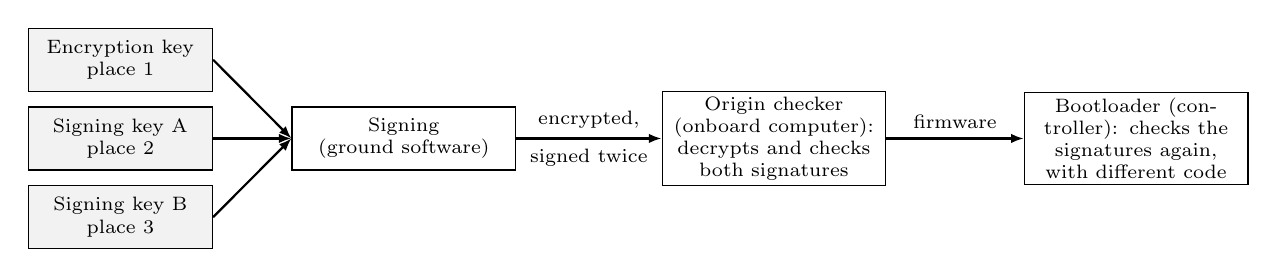
\begin{tikzpicture}[font=\scriptsize,
  box/.style={draw, text width=2.7cm, align=center, minimum height=0.8cm, inner sep=2pt},
  key/.style={box, fill=black!5, text width=2.2cm},
  ar/.style={-{Latex[length=1.6mm]}, thick}]
\node[key] (k1) at (0,1.0) {Encryption key\\place 1};
\node[key] (k2) at (0,0) {Signing key A\\place 2};
\node[key] (k3) at (0,-1.0) {Signing key B\\place 3};
\node[box] (sg) at (3.6,0) {Signing\\(ground software)};
\node[box] (oc) at (8.3,0) {Origin checker (onboard computer): decrypts and checks both signatures};
\node[box] (ss) at (12.9,0) {Bootloader (controller): checks the signatures again, with different code};
\foreach \k in {k1,k2,k3} \draw[ar] (\k.east) -- (sg.west);
\draw[ar] (sg) -- node[above]{encrypted,} node[below]{signed twice} (oc);
\draw[ar] (oc) -- node[above]{firmware} (ss);
\end{tikzpicture}
\caption{Proof of origin. Each key is kept in its own place, so one disclosed
key is not enough. Commands stop at the onboard computer's check; firmware is
checked again on the controller.}
\label{fig:origin}
\end{figure}

\field{Adds}
\begin{itemize}
\item Every command and firmware image shall be encrypted from the ground
  software to the onboard computer software [11,~Sec.~4.1.1, p.~9].
\item Every command and firmware image shall carry two signatures, made with
  two keys kept apart from each other and from the encryption key.
\item The onboard computer software shall act on a command or firmware image
  only when it decrypts and both signatures are valid.
\item The controller firmware shall check firmware signatures with code
  different from the onboard computer software's.
\end{itemize}

% ---------------------------------------------------------------- 5.5
\needspace{9\baselineskip}
\subsection{Two Clocks}
\label{sec:clocks}
\field{Problem} Expiry, arm time-outs, scheduled commands, time-tags and the
trial time limit all depend on the onboard clock. A wrong clock alone runs a
scheduled command at the wrong time and gives reports wrong times
[5,~Sec.~5.2]. Targets H-6, here a scheduled command run at the wrong time,
and H-9, here reports shown with wrong times.

\smallskip
{\small\noindent\begin{tabularx}{\textwidth}{@{}l>{\raggedright\arraybackslash}Xccc@{}}
\toprule
 & Option & \sev{H-6}{CRITICAL} & \sev{H-9}{CRITICAL} & Chosen \\
\midrule
a & One clock, compared with ground time only at contacts [6,~REQ-072]. Between contacts, a wrong clock runs scheduled commands at the wrong time and stamps wrong times on reports, and nothing notices. & 1 & 1 & NO \\
b & Report and command numbers replace times where possible. The order of reports survives a wrong clock, but scheduled commands and time-tags still need it. & 1 & 1 & NO \\
c & A second clock in the controller, with its own time source and set only from ground time. A scheduled command runs only when both clocks agree, and every report carries both times, so one wrong clock is caught by the other. A wrong ground time reaches both clocks; the ground software's check of every command before it is sent [6,~REQ-089] keeps that case at two failures, and a wrong time that passes it is an accepted risk. & 2 & 2 & YES \\
\bottomrule
\end{tabularx}}


\field{Choice} Option c \tbr{clocks}, shown in Figure~\ref{fig:clocks}.

\begin{figure}[H]
\centering
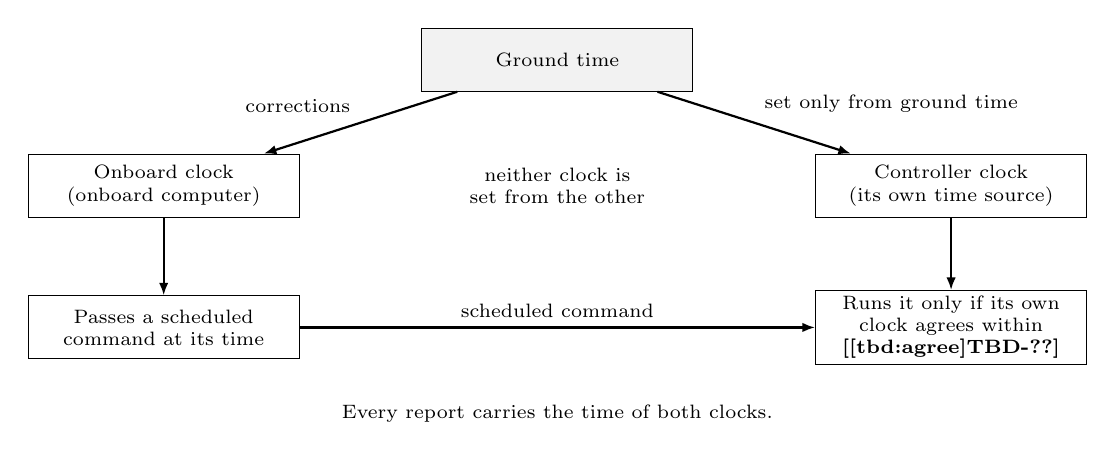
\begin{tikzpicture}[font=\scriptsize,
  box/.style={draw, text width=3.3cm, align=center, minimum height=0.8cm, inner sep=2pt},
  ar/.style={-{Latex[length=1.6mm]}, thick}]
\node[box, fill=black!5] (gt) at (5,1.6) {Ground time};
\node[box] (oc) at (0,0) {Onboard clock\\(onboard computer)};
\node[box] (cc) at (10,0) {Controller clock\\(its own time source)};
\draw[ar] (gt) -- node[above left]{corrections} (oc);
\draw[ar] (gt) -- node[above right]{set only from ground time} (cc);
\node[align=center] at (5,0) {neither clock is\\set from the other};
\node[box] (oc2) at (0,-1.8) {Passes a scheduled command at its time};
\node[box] (cc2) at (10,-1.8) {Runs it only if its own clock agrees within \tbd{agree}};
\draw[ar] (oc) -- (oc2);
\draw[ar] (cc) -- (cc2);
\draw[ar] (oc2) -- node[above]{scheduled command} (cc2);
\node[align=center] at (5,-2.9) {Every report carries the time of both clocks.};
\end{tikzpicture}
\caption{Two clocks. Neither is set from the other, so one wrong value cannot
reach both.}
\label{fig:clocks}
\end{figure}

\field{Adds}
\begin{itemize}
\item The controller firmware shall keep its own clock, from a time source
  separate from the onboard computer's.
\item The controller's clock shall be set only from ground time.
\item The controller firmware shall refuse a command past its expiry, by its
  own clock.
\item The controller firmware shall run a scheduled command only when its own
  clock agrees with the scheduled time within \tbd{agree}.
\item Every report shall carry the time of both clocks.
\end{itemize}

% ---------------------------------------------------------------- 5.6
\needspace{9\baselineskip}
\subsection{Held Data}
\label{sec:held}
\field{Problem} A bit error can change a held command, the arm state or the
kept data after its check and before its use (A-5) [5,~Sec.~5.2]. Targets H-6,
here a command acted on in a form the operator did not intend.

\smallskip
{\small\noindent\begin{tabularx}{\textwidth}{@{}l>{\raggedright\arraybackslash}Xcc@{}}
\toprule
 & Option & \sev{H-6}{CRITICAL} & Chosen \\
\midrule
a & Each item is checked once, on arrival. A bit error afterwards goes unnoticed. & 1 & NO \\
b & Each held item carries a check value and is checked again just before use; the arm state is stored as a pattern that no single bit error turns into armed. A bit error now has to produce a matching check value as well. & 2 & YES \\
c & Memory hardware that corrects bit errors on its own. Also two failures, but it depends on a hardware feature. & 2 & NO \\
\bottomrule
\end{tabularx}}


\field{Choice} Option b \tbr{held}. MCUboot notes the same risk: skipping the check
before use lets an image changed after a good check run unchecked
[9,~Sec.~Integrity Check]. Unlike option c, option b needs no hardware
feature; option c can be added where the hardware has it.

\field{Adds}
\begin{itemize}
\item Every held command and the kept data shall be stored with a check value
  and checked just before use.
\item The arm state shall be stored so that no single bit error makes it armed.
\end{itemize}

% ---------------------------------------------------------------- 5.7
\needspace{9\baselineskip}
\subsection{Two Kinds of Connection}
\label{sec:links}
\field{Problem} The two data-link connections share software at both ends, so
one defect cuts both (R-1) [5,~Sec.~5.2]. Targets H-4, the controller no
longer commanded or observed. The count is of failures that cut both
connections at once.

\smallskip
{\small\noindent\begin{tabularx}{\textwidth}{@{}l>{\raggedright\arraybackslash}Xcc@{}}
\toprule
 & Option & Failures to cut both & Chosen \\
\midrule
a & Two connections of one kind share one driver at each end. One defect in that driver cuts both. & 1 & NO \\
b & Each connection has its own driver, but both are of one kind. A fault common to that kind, in its design or in its handling, cuts both. & 1 & NO \\
c & Two different kinds, each with its own driver. Cutting both takes a separate failure in each. & 2 & YES \\
\bottomrule
\end{tabularx}}


\field{Choice} Option c \tbr{links}. One connection carries on when the other is
cut (O-3). H-4 still falls to the loss of the onboard computer (R-4).

\field{Adds}
\begin{itemize}
\item The two data-link connections shall be of different kinds.
\end{itemize}

% ===========================================================================
% ===========================================================================
\section{Components}
\label{sec:components}
Each component, its role, and the requirements it meets [2,~Sec.~3.3].
Every requirement [6,~Secs.~4.0--7.0] is met by at least one component;
requirements that the decisions add are allocated when they enter the
requirements.

All components are safety-critical [7,~Sec.~4.0] and new code, except the
bootloader, the origin checker and signing, which are built around a
published cryptographic library.

The components from the mode manager to the data-link drivers form the main
firmware; the controller keeps two copies of it. Figure~\ref{fig:startup}
shows which copy runs in each controller mode [4,~Sec.~3.4].

\needspace{12\baselineskip}
{\footnotesize
\begin{xltabular}{\textwidth}{@{}>{\raggedright\arraybackslash}p{2.6cm}>{\raggedright\arraybackslash}X>{\raggedright\arraybackslash}p{3.6cm}@{}}
\toprule
Component & Role & Requirements \\
\midrule
\endhead
\multicolumn{3}{@{}l}{\textit{Controller firmware}} \\
Bootloader & Runs first at every start. Sets a safe state, checks each firmware copy for damage and origin, counts failed starts, and starts the new, previous or last-resort firmware. & REQ-004~to~006, REQ-013~to~019, REQ-023, REQ-113 \\
Mode manager & Holds the controller mode, runs the trial, and confirms new firmware or gives it up. & REQ-001~to~003, REQ-011~to~013, REQ-020, REQ-021, REQ-024~to~026, REQ-113, REQ-117 \\
Command checker & Checks every command for mode, values, arming, expiry and repeats; checks held commands again before running them; answers and logs. & REQ-027~to~036, REQ-100 \\
Update receiver & Stores new firmware in the free copy, never over the previous or last-resort firmware. & REQ-007, REQ-008 \\
Health monitor & Tests the controller, detects faults, restarts it when it stops responding, and sends health and event reports. & REQ-022, REQ-037~to~041 \\
Controller clock & Keeps the controller's own time, set only from ground time. & REQ-030 \\
Data-link drivers & One driver for each data-link connection, sharing no code. & REQ-042, REQ-099 \\
Last-resort firmware & A separate program sharing no code or kept data with the others. Sets a safe state, answers commands, sends reports, and receives new firmware. & REQ-004, REQ-009, REQ-010 \\
\multicolumn{3}{@{}l}{\textit{Onboard computer software}} \\
Command gate & Checks every command for origin, newness, expiry and arming, passes it on, and logs it. & REQ-064~to~067, REQ-087, REQ-100, REQ-112 \\
Origin checker & Decrypts commands and firmware, checks their two signatures, and replaces the means of checking them on command. & REQ-043, REQ-064, REQ-084~to~086 \\
Scheduler & Holds scheduled commands and passes each on once, at its run time, across restarts. & REQ-068, REQ-069 \\
Update manager & Checks new firmware, stores it, and delivers it over the data link, resuming after any interruption. & REQ-043~to~053, REQ-063 \\
Report store & Checks, numbers and time-tags every report, stores reports between contacts, and sends them at the next one. & REQ-070, REQ-071, REQ-074~to~079 \\
Clock keeper & Compares the onboard clock with ground time and applies corrections. & REQ-072, REQ-073 \\
Controller watch & Notices a silent controller, restarts it, and calls the restore when no firmware runs. & REQ-061 \\
Supervisor & Restarts any program of the onboard computer software that crashes. & REQ-062 \\
Data-link drivers & One driver for each data-link connection, sharing no code. & REQ-080~to~082, REQ-099 \\
Reprogramming drivers & One driver for the controller's debug port and one for its factory loader, sharing no code. & REQ-054, REQ-058, REQ-059, REQ-083 \\
Restore program & A separate program with its own firmware store. Restores the controller through the reprogramming drivers, loads firmware from the ground through them, and checks its store and both ways in between uses. & REQ-054~to~060, REQ-083 \\
\multicolumn{3}{@{}l}{\textit{Ground software}} \\
Operator console & Lets only the operator in, and shows reports, unanswered commands and the running firmware. & REQ-091, REQ-094, REQ-095 \\
Command builder & Builds every command from the shared command list and checks it before it is sent. & REQ-089, REQ-100 \\
Signing & Encrypts and signs every command and firmware image with three keys kept in separate places, and keeps a recoverable copy of the means of proving origin. & REQ-088, REQ-096 \\
Release checker & Checks every firmware release before signing, and the signed image before it is sent, with the checks the onboard computer makes. & REQ-090, REQ-114 \\
Report archive & Keeps every report received and checks it for damage. & REQ-092, REQ-093 \\
Contact planner & Plans commands, uploads and report retrieval for coming contacts, and sends a planned command sequence, stopping at the first command refused or not answered. & REQ-097, REQ-115, REQ-116 \\
\multicolumn{3}{@{}l}{\textit{All software items}} \\
Every component & Rules that apply to all software. & REQ-098, REQ-101~to~111 \\
\bottomrule
\end{xltabular}}
% ===========================================================================
\needspace{12\baselineskip}
\section{Interfaces}
Each interface is specified byte by byte before any code is written.
Interfaces between components of one software item are set in its detailed
design.

\smallskip
{\small\noindent\begin{tabularx}{\textwidth}{@{}l>{\raggedright\arraybackslash}p{4.6cm}>{\raggedright\arraybackslash}X@{}}
\toprule
Interface & Between & Carries \\
\midrule
Operator interface & Operator and ground software & The operator's decisions; reports and the System's state \\
Radio link & Ground software and onboard computer software & Signed commands and firmware; answers and reports \\
Data link A & Onboard computer and controller & Commands, answers, reports and firmware \\
Data link B & Onboard computer and controller & The same as data link A, over a different kind of connection \\
Reprogramming link A & Reprogramming drivers and controller & The controller's debug port: its restart, and memory writes with the processor stopped \\
Reprogramming link B & Reprogramming drivers and controller & The controller's factory loader: started by a boot pin, it accepts new firmware \\
\bottomrule
\end{tabularx}}

% ===========================================================================
\section{Hardware Needs}
\label{sec:hardware}
The hardware must provide what the decisions above assume. Each need is
checked against the two boards before this document is released \tbd{boards}.

\smallskip
{\small\noindent\begin{tabularx}{\textwidth}{@{}>{\raggedright\arraybackslash}Xl@{}}
\toprule
Need & Needed by \\
\midrule
A debug port that writes the controller's memory whatever it holds & Section~\ref{sec:wayback} \\
A factory loader in the controller that firmware cannot change, started by a boot pin & Section~\ref{sec:wayback} \\
Wires from the onboard computer to the controller's reset and boot pins & Section~\ref{sec:wayback} \\
No way for controller firmware to disable the debug port or the factory loader & Section~\ref{sec:wayback} \\
A way for the restore to make the last-resort firmware run first & Section~\ref{sec:startup} \\
Room in the controller for the bootloader, two main firmware copies, the last-resort firmware and the kept data & Section~\ref{sec:startup} \\
Kept data in the controller that survives a restart and a power loss & REQ-017 \\
Room on the onboard computer for two separate firmware stores & Section~\ref{sec:apart} \\
Processing in the controller to check two signatures within the restart time & Section~\ref{sec:origin}; REQ-023 \\
A time source in the controller separate from the onboard computer's & Section~\ref{sec:clocks} \\
Two different kinds of connection between the onboard computer and the controller & Section~\ref{sec:links} \\
\bottomrule
\end{tabularx}}

% ===========================================================================
\appendix
\renewcommand{\thesection}{\Alph{section}}
\renewcommand{\thesubsection}{\Alph{section}.\arabic{subsection}}

\section{Open Items}
The values below are not yet known.
\begin{description}
\tbditem{ref}{Project name and document reference.}
\tbditem{agree}{Largest allowed difference between the controller's clock and
  the time of a scheduled command.}
\tbditem{boards}{Check of each hardware need against the two boards.}
\end{description}

\medskip
\noindent The proposals below await the author's acceptance.
\begin{description}
\tbritem{wayback}{The way back in: option c (Section~\ref{sec:wayback}).}
\tbritem{apart}{Restore apart from update: option b (Section~\ref{sec:apart}).}
\tbritem{origin}{Proof of origin: option d (Section~\ref{sec:origin}).}
\tbritem{clocks}{Two clocks: option c (Section~\ref{sec:clocks}).}
\tbritem{held}{Held data: option b (Section~\ref{sec:held}).}
\tbritem{links}{Two kinds of connection: option c (Section~\ref{sec:links}).}
\end{description}

\medskip
\noindent The author accepted, on 11 October 2026, option c of
Section~\ref{sec:startup} and the risk of a wrong ground time that passes the
ground software's check (Section~\ref{sec:clocks}).

\end{document}
